\documentclass{beamer}
\mode<presentation>
\setbeamertemplate{navigation symbols}{}

% ----------------------------------------------------------------------
%footer
\setbeamertemplate{footline}
{
  \leavevmode
    \hfill
    \usebeamerfont{footer}
    ~~~~~~~~~~~~~~~~~~~~~~~~~~~~~~~~~~
    ~~~~~~~~~~~~~~~~~~~~~~~~~~~~~~~~~~
    \insertframenumber{} / \inserttotalframenumber
    ~~~~~
}

\usepackage[utf8]{inputenc}
\usepackage[T1]{fontenc}
\usepackage[french]{babel}

%figures
\usepackage{graphicx}
\graphicspath{{fig/}}
\DeclareGraphicsExtensions{.eps,.pdf,.jpg,.png}
\usepackage{tikz}

%math
\usepackage{amssymb}
\usepackage{amsmath}
\usepackage{cancel}

% ----------------------------------------------------------------------
%macros

\newcommand{\Z}{{\ensuremath\mathbb{Z}}}
\newcommand{\N}{{\ensuremath\mathbb{N}}}
\newcommand{\R}{{\ensuremath\mathbb{R}}}

%%\renewcommand{\vec}[1]{\mathbf{#1}}
%%\newcommand{\ve}[1]{\ensuremath{\vec{e}_{#1}}}

\DeclareMathOperator*{\argmin}{arg\,min}

\newcommand{\cat}{
  \begin{tikzpicture}[baseline=-1mm]
    \node at (0,0) {
\includegraphics[width=1cm]{cat.png}};
  \end{tikzpicture}
}
% ----------------------------------------------------------------------
\title[]
 {4TC-IAT, Optimisation}

\author[T. Roussillon]
 {Tristan Roussillon}

\date{2025}

\institute{INSA Lyon, TC}

\begin{document}

% ----------------------------------------------------------------------
\begin{frame}
  \titlepage
\end{frame}

% ----------------------------------------------------------------------
\section{Introduction}
% ----------------------------------------------------------------------

%% % ----------------------------------------------------------------------
%% \begin{frame}
%%   \frametitle{Exemples (1/3)}

%% \begin{block}{Moyenne des $\{v_i\}_{i=1,\dots,m}$ : }
%%   \[ \frac{1}{m} \sum_{i=1}^{m} v_i = \min_x \sum_{i=1}^{m} (x - v_i)^2. \]
%% \end{block}

%% \begin{block}{Apprentissage supervisé : }
%%   \begin{itemize}
%%   \item fonction de prédiction $f$(\cat) = cat, 
%%   \item \[ \min_f \sum_\text{ensemble d'apprentissage} (\text{erreur de prédiction de } f). \]
%%   \end{itemize}
%% \end{block}

%% \end{frame}

%% % ----------------------------------------------------------------------
%% \begin{frame}
%%   \frametitle{Exemples (2/3)}

%%   \begin{block}{Flot maximum : }
%%     \centering
%%     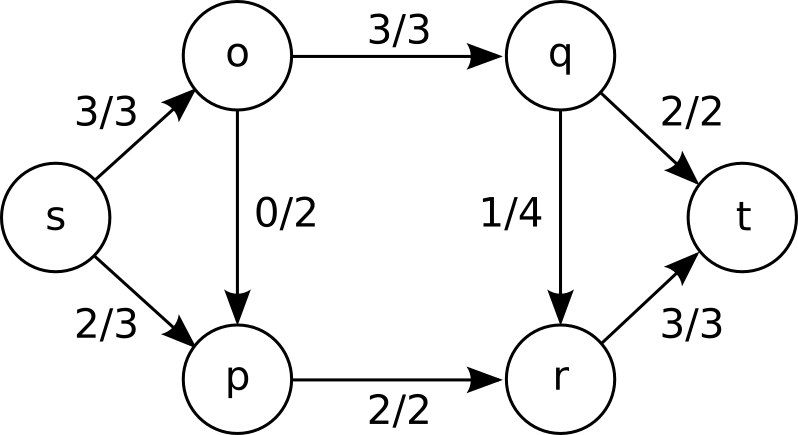
\includegraphics[width=3cm]{max-flow.png}
%%   \end{block}
  
%%   \begin{block}{Plus courts chemins : }
%%     \centering
%%     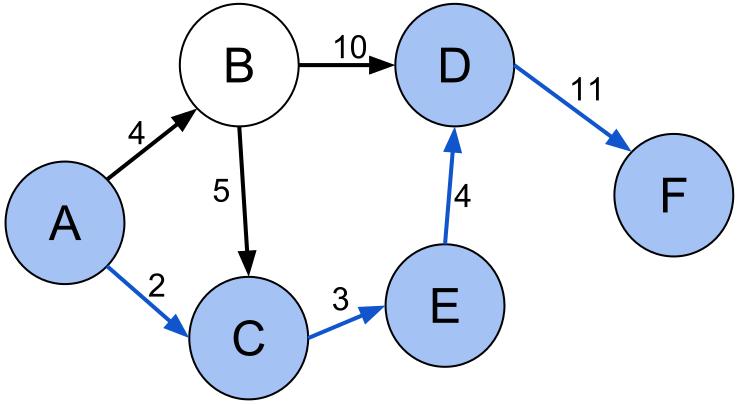
\includegraphics[width=3cm]{shortest-path.png}
%%   \end{block}

%% \end{frame}

%% % ----------------------------------------------------------------------
%% \begin{frame}
%%   \frametitle{Exemples (3/3)}
  
%%   \begin{block}{Séparation linéaire avec marge maximale : }
%%     \centering
%%     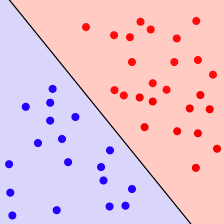
\includegraphics[width=2cm]{linear-separation.png}
%%   \end{block}
  
%%   \begin{block}{Plus petit cercle englobant : }
%%     \centering
%%     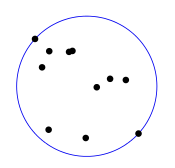
\includegraphics[width=2cm]{seb.png}
%%   \end{block}
  
%% \end{frame}
%% % ----------------------------------------------------------------------
%% \begin{frame}
%%   \frametitle{Introduction}

%%   \begin{block}{Les problèmes d'optimisation sont fréquents}
%%   \begin{itemize}
%%   \item à la question ``y a-t-il une solution ?'' (existence)\\
%%     suit ``quelle est la meilleure solution ?'' (optimisation)
%%   \item l'optimisation peut être sous-jacente : par ex., en apprentissage supervisé, on cherche
%%     une fonction de prédiction qui minimise l'erreur de prédiction exprimée comme une fonction de coût.
%%   \item certains problèmes sont difficiles et requièrent des méthodes inhabituelles pour découvrir
%%     des solutions, mêmes approchées : c'est une partie de ce qu'on appelle l'IA.
%%   \end{itemize}
%%   \end{block}
  
%% \end{frame}

% ----------------------------------------------------------------------
\begin{frame}
  \frametitle{Problèmes d'optimisation que vous connaissez}

  \begin{block}{Plus court chemin : }
    \centering
    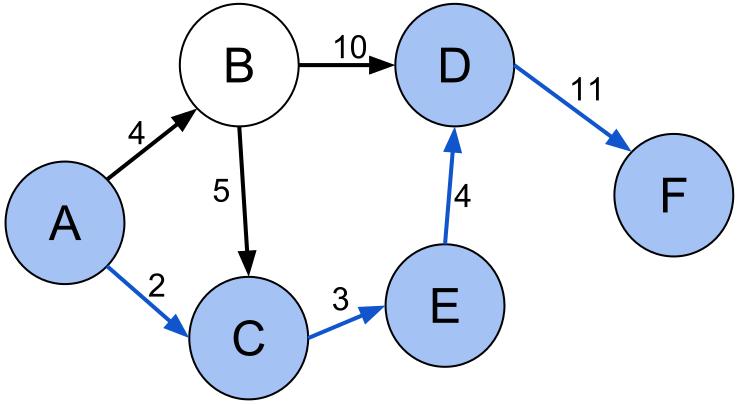
\includegraphics[width=3cm]{shortest-path.png}
  \end{block}

  \begin{block}{Flot maximum : }
    \centering
    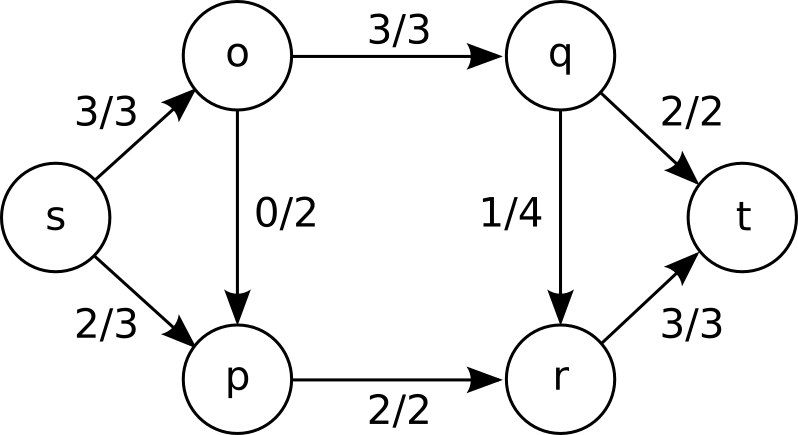
\includegraphics[width=3cm]{max-flow.png}
  \end{block}
  
  \begin{block}{Plus petit cercle englobant : }
    \centering
    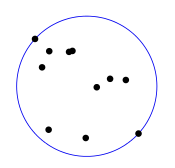
\includegraphics[width=2cm]{seb.png}
  \end{block}
  
\end{frame}


% ----------------------------------------------------------------------
\begin{frame}
  \frametitle{Problèmes d'optimisation en télécommunications}

  \begin{itemize}
  \item Allocation de fréquences / channel assignment
    %Global System for Mobile Communications (GSM) (historiquement « Groupe spécial mobile »1)
    %est une norme numérique de seconde génération pour la téléphonie mobile
  \item Allocation de canaux / time slot assignment
    %% Le time division multiple access (TDMA) ou accès multiple à répartition dans le temps en français, est une technique de contrôle d'accès au support permettant de transmettre plusieurs flux de trafic sur un seul canal ou une seule bande de fréquence. Il utilise une division temporelle de la bande passante, dont le principe est de répartir le temps disponible entre les différents utilisateurs. Par ce moyen, une fréquence (porteuse) ou une longueur d'onde peut être allouée, à tour de rôle (quasi simultanément), à plusieurs abonnés. 
  \item Routage et allocation de longueurs d'onde / routing and wavelength assignment
    %multiplexage en longueur d'onde, souvent appelé WDM (Wavelength Division Multiplexing en anglais)
  \item Routage IP
  \item Optimisation dans les réseaux radio maillés :
    \begin{itemize}
    \item placement min. de points d'accès / min. gateway placement
    \item placement équitable de points d'accès / fair gateway placement
    \item routage équitable / fair joint routing and scheduling
    \item routage en temps minimum / minimum time routing
    \end{itemize}
    %p. 36/37 thèse Optimisation de la capacité des réseaux maillés, C. Molle  
  \end{itemize}
  
\end{frame}

% ----------------------------------------------------------------------
\begin{frame}
  \frametitle{Optimisation et IA}

  \begin{block}{Problème \emph{complexe}}
  \begin{itemize}
  \item IA $\approx$ faire résoudre par une machine un problème \emph{complexe}
  \item problème \emph{complexe} $\approx$ problème d'optimisation (y a-t-il une solution ?
    quelle est la meilleure solution ?)
  \end{itemize}
  \end{block}

  \begin{block}{Apprentissage automatique}
    \begin{itemize}
    \item apprentissage supervisé
      \begin{itemize}
      \item fonction de prédiction $f$(\cat) = chat, 
      \item trouver $f$ qui minimise \[ \sum_\text{ensemble d'apprentissage} (\text{erreur de prédiction de } f). \]
      \end{itemize}
    \end{itemize}
  \end{block}

\end{frame}

% ----------------------------------------------------------------------
\begin{frame}
  \frametitle{Ce qu'est l'optimisation en une image}

  \begin{exampleblock}{Exemple dans $\R$}
    \centering
    \includegraphics[width=0.7\textwidth,page=1]{opt-loc}
  \end{exampleblock}

\end{frame}

% ----------------------------------------------------------------------
\begin{frame}
  \frametitle{Formulation mathématique}

  \[
  \text{(P)} \left\{
  \begin{array}{c}
    \text{trouver} \ x \ \text{qui minimise} \ f(x) \ \text{tel que :} \\
    g_i(x) \leq 0, \ i \in I = \{1, \dots, m\} \\
    x \in S \subseteq \R^n
  \end{array}
  \right.
  \]

  \only<1>{
    \begin{block}{Vocabulaire}
    \begin{itemize}
    \item fonction objectif : $f : \R^n \rightarrow \R$
    \item inconnues : composantes du vecteur $x := (x_1, \dots, x_n) \in \R^n$
    \item contraintes : $g_i(x) \leq 0$ et $x \in S$
    \item une solution (candidate) : $x$ satisfaisant les contraintes
    \item solution optimale/optimum global : une solution minimisant $f$
    \end{itemize}
    %distinction des contraintes en deux:
    %- generalisation a plusieurs classes de pb
    %- traites differement dans les algos
    \end{block}
  }
  \only<2>{
    \begin{block}{Remarques}
    \begin{itemize}
    \item max $f'$ $\Leftrightarrow$ min $-f'$
    \item nombre d'inconnues $n \geq 1$ 
    \item nombre de contraintes $m \geq 0$
    \item contraintes d'égalité $g'(x) = 0$ $\Leftrightarrow$ $g'(x) \leq 0$
      et $-g'(x) \leq 0$
    \item généralement pas d'inégalités strictes
    \end{itemize}
    \end{block}
    %existence de solution (th. de Weierstrass)
    %si f est une fonction reelle continue sur K \subset R^n ferme et borne, alors il existe
    %une solution optimale x \in K qui min f(x)
    %existence aussi si f est une fonction reelle continue et possède la propriété de croissance à l'infini:
    %f(x) -> +inf qs x -> +inf
    %inégalités strictes => ensemble de solutions non ferme et borne, donc possiblement pas de solutions. 
  }
  \only<3>{
    \begin{block}{Résoudre (P) peut être difficile...}
    \begin{itemize}
    \item ensemble des solutions vide, très grand, voire infini
    \item problème non borné 
    \item $n, m$ grands
    \item $f$ et $g_i$ quelconques, $f$ non analytiquement connu %ni differentiable, ni convexe, ni lineaire
    %%\item $f$ peut être (quasiment) plat autour du min
      %si plat, plusieurs solutions optimales, si quasiment, instabilités numériques 
    \item cas discret ($S = \Z^n$), NP-complet 
    \end{itemize}
    \end{block}
  }

  \only<4->{
    \begin{block}{Résoudre (P) peut être facile...}
    \begin{itemize}
    \item cas continu
    \item problème borné
    \item une solution
    \item $f$ connu < différentiable < convexe
    \item aucune contrainte ou des contraintes linéaires
    \end{itemize}
    \end{block}
  }
\end{frame}

% ----------------------------------------------------------------------
\section{Convexité et différentiabilité}
% ----------------------------------------------------------------------
%permet de dire si on peut chercher un min ou un max
%permet de dire si tout optimum local est un optimum global ou non

% ----------------------------------------------------------------------
\begin{frame}<beamer>
  \frametitle{Sommaire}
  \tableofcontents[currentsection]
\end{frame}

% ----------------------------------------------------------------------
\begin{frame}
  \frametitle{Convexité d'un ensemble}

  \begin{block}{Définition}
    $S \subset \R^n$ est convexe ssi  
    pour tout $x,y \in S$ et $\lambda \in [0,1]$,
    $\lambda x - (1 - \lambda) y \in S$. 
  \end{block}

  \begin{exampleblock}{Exemple pour $S \subset \R^2$}
    \centering
    \includegraphics[width=0.25\textwidth,page=2]{ens-conv}\hspace{0.05\textwidth}
    \includegraphics[width=0.25\textwidth,page=1]{ens-conv}
  \end{exampleblock}
  
\end{frame}

% ----------------------------------------------------------------------
\begin{frame}
  \frametitle{Contrôle}

  \includegraphics<+>[width=1\textwidth]{ens-conv-Q}%
  \includegraphics<+>[width=1\textwidth]{ens-conv-A}%

  \scriptsize{\url{https://www.youtube.com/playlist?list=PL9_jI1bdZmz0hIrNCMQW1YmZysAiIYSSS}}
\end{frame}

% ----------------------------------------------------------------------
\begin{frame}
  \frametitle{Convexité d'une fonction}

  \begin{block}{Définition}
     Soit $S \subset \R^n$ convexe.
     Une fonction $f : S \rightarrow \R$ est convexe ssi  
    pour tout $x,y \in S$ et $\lambda \in [0,1]$,
    $f(\lambda x - (1 - \lambda) y) \leq \lambda f(x) + (1 - \lambda) f(y)$. 
  \end{block}

  \begin{exampleblock}{Exemple pour $f:\R \rightarrow \R$}
    \centering
    \includegraphics[width=0.45\textwidth,page=2]{fonc-conv}\hspace{0.05\textwidth}
    \includegraphics[width=0.45\textwidth,page=1]{fonc-conv}
  \end{exampleblock}
  
\end{frame}

% ----------------------------------------------------------------------
\begin{frame}
  \frametitle{Différentiabilité pour $f: \R \rightarrow \R$ (1/2) }

  \begin{block}{Dérivée première}
    \begin{columns}
      \begin{column}{0.5\textwidth}
        \begin{align*}
          f'(x) &:= \frac{\partial f}{\partial x}(x) \\
          &= \lim_{h \rightarrow 0} \frac{f(x+h) - f(x)}{h}.
        \end{align*}
      \end{column}
      \begin{column}{0.5\textwidth}
        \begin{center}
          \includegraphics<+>[width=1\textwidth,page=2]{derivee}%    
          \includegraphics<+>[width=1\textwidth,page=1]{derivee}%
          \includegraphics<+>[width=1\textwidth,page=3]{derivee}%
        \end{center}
      \end{column}
    \end{columns}
  \end{block}

  \begin{block}{Interprétation en un point $x^0$}
    \begin{itemize}
    \item Le signe de $f'(x^0)$ indique comment évolue $f$ autour de $x^0$: 
      \begin{itemize}
      \item \alert<1-2>{si $f'(x^0) < 0$, $f$ $\downarrow$ quand $x^0$ $\uparrow$},
      \item si $f'(x^0) > 0$, $f$ $\uparrow$ quand $x^0$ $\uparrow$,
      \end{itemize}
    \item La valeur absolue donne la \emph{vitesse} du changement. 
      \begin{itemize}
      \item \alert<3>{si $f'(x^0) = 0$, $f$ change \emph{peu} autour de $x^0$}. 
      \end{itemize}
    \end{itemize}
  \end{block}
  
\end{frame}

% ----------------------------------------------------------------------
\begin{frame}
  \frametitle{Différentiabilité pour $f: \R \rightarrow \R$ (2/2) }

  \begin{block}{Dérivée seconde = dérivée de la dérivée première}
    $f'' := \frac{\partial f'}{\partial x} = \frac{\partial ^{2}f}{\partial x^{2}}$.
  \end{block}

  \begin{block}{Interprétation en un point $x^0$}
    \begin{itemize}
    \item Le signe de $f''(x^0)$ indique comment évolue $f'$ autour de $x^0$. 
      \begin{itemize}
      \item si $f''(x^0) < 0$, $f'$ $\downarrow$ quand $x^0$ $\uparrow$,
      \item si $f''(x^0) > 0$, $f'$ $\uparrow$ quand $x^0$ $\uparrow$,
      \end{itemize}
    \end{itemize}
  \end{block}

  \begin{block}{En particulier, si $f'(x^0) = 0$ et $f''(x^0) > 0$, alors}
    \begin{itemize}
      \item $f'$ $\uparrow$ (donc $f'$ positive et $f$ $\uparrow$) quand $x^0$ $\uparrow$,
      \item $f'$ $\downarrow$ (donc $f'$ négative et $f$ $\downarrow$) quand $x^0$ $\downarrow$. 
    \end{itemize}
    \alert<2->{En quoi cela peut nous aider à trouver $x^\star$ qui minimise $f$ ?}
  \end{block}
  
\end{frame}

% ----------------------------------------------------------------------
\begin{frame}
  \frametitle{Exemples numériques pour $f:\R \rightarrow \R$}

  \begin{block}{$f(x) = x^2 - 6x + 4$}
    \begin{itemize}
      \item $f'(x) =$\only<1>{?}\only<2>{$2x - 6$}
      \item $f''(x) =$ \only<1>{?}\only<2>{$2$}
    \end{itemize}
  \end{block}

  \begin{block}{$f(x) = 2x^3 - x^2 + 2x + 5$}
    \begin{itemize}
      \item $f'(x) =$\only<1>{?}\only<2>{$6x^2 - 2x + 2$}
      \item $f''(x) = $\only<1>{?}\only<2>{$12x - 2$}
    \end{itemize}
  \end{block}
  
\end{frame}

% ----------------------------------------------------------------------
\begin{frame}
  \frametitle{Différentiabilité pour $f: \R^n \rightarrow \R$ (1/2)}
  
  \begin{block}{Gradient (vecteur), extension de la dérivée première}
    ${\nabla f} := (\frac{\partial f}{\partial x_1}, \frac{\partial f}{\partial x_2}, \dots, \frac{\partial f}{\partial x_n})$ \\
    \begin{itemize}
    \item Il donne la direction dans laquelle $f$ augmente
    \item (et est perpendiculaire à la courbe de niveau projetée),
    \item sa magnitude donne la vitesse du changement. 
    \end{itemize}
  \end{block}

  \begin{center}
    \includegraphics<+>[width=0.9\textwidth]{gradient}    
  \end{center}
  
\end{frame}

% ----------------------------------------------------------------------
\begin{frame}
  \frametitle{Différentiabilité pour $f: \R^n \rightarrow \R$ (2/2)}
  
  \begin{block}{Hessien (matrice), extension de la dérivée seconde}
    $\nabla^2 f :=
    \begin{bmatrix}{\frac {\partial ^{2}f}{\partial x_{1}^{2}}}&{\frac {\partial ^{2}f}{\partial x_{1}\partial x_{2}}}&\cdots &{\frac {\partial ^{2}f}{\partial x_{1}\partial x_{n}}}\\{\frac {\partial ^{2}f}{\partial x_{2}\partial x_{1}}}&{\frac {\partial ^{2}f}{\partial x_{2}^{2}}}&\cdots &{\frac {\partial ^{2}f}{\partial x_{2}\partial x_{n}}}\\\vdots &\vdots &\ddots &\vdots \\{\frac {\partial ^{2}f}{\partial x_{n}\partial x_{1}}}&{\frac {\partial ^{2}f}{\partial x_{n}\partial x_{2}}}&\cdots &{\frac {\partial ^{2}f}{\partial x_{n}^{2}}}\end{bmatrix}$
  \end{block}

  \begin{block}{Matrice (semi-)définie positive, extension du signe}
    Une matrice semi-définie positive (resp. définie positive) si 
    ses valeurs propres sont $\geq 0$ (resp. $> 0$).
  \end{block}

  \only<1>{
    \begin{block}{Note 1 : }
    Les valeurs propres d'une matrice carrée $M$ sont les composantes du vecteur
    $\lambda^T := (\lambda_1, \lambda_2,\dots, \lambda_n)$, solutions de
    l'équation $\det{(\lambda I - M)} = 0$.  
  \end{block}
  }
  \only<2>{
    \begin{block}{Note 2 :}
    \begin{tabular}{ccc}
      hessien & $\Leftrightarrow$ & dérivée seconde \\\hline
      semi-définie positive & $\Leftrightarrow$ & $\geq 0$ \\\hline
      définie positive & $\Leftrightarrow$ & $> 0$  
    \end{tabular}
  \end{block}
  }
\end{frame}

% ----------------------------------------------------------------------
\begin{frame}
  \frametitle{Exemple numérique pour $f:\R^2 \rightarrow \R$}

  \begin{block}{$f(x_1,x_2) = x_1^2 + x_2^2 - 4x_1 + 8x_2 - 5$}
    \only<1-2>{
      Dérivées partielles : 
      \begin{itemize}
      \item $\frac{\partial f}{\partial x_1} = $\only<1>{?}\only<2>{$2x_1 - 4$},
      \item $\frac{\partial f}{\partial x_2} = $\only<1>{?}\only<2>{$2x_2 + 8$},
      \item $\frac{\partial^2 f}{\partial x_1^2} = $\only<1>{?}\only<2>{$2$},
      \item $\frac{\partial^2 f}{\partial x_1x_2} = $\only<1>{?}\only<2>{$0$},
      \item $\frac{\partial^2 f}{\partial x_2x_1} = $\only<1>{?}\only<2>{$0$},
      \item $\frac{\partial^2 f}{\partial x_2^2} = $\only<1>{?}\only<2>{$2$}.
      \end{itemize}
    }
    \only<3-4>{
      gradient, hessien : 
      \begin{itemize}
      \item ${\nabla f}(x_1,x_2) =$\only<3>{?}
        \only<4>{$\left(\begin{array}{l}
            2x_1 - 4\\
            2x_2 + 8
          \end{array}
          \right)$}
      \item $\nabla^2f(x_1,x_2) =$\only<3>{?}
        \only<4>{$\left(\begin{array}{cc}
            2 & 0 \\
            0 & 2 \\
          \end{array}
          \right)$}
      \end{itemize}
    }
  \end{block}
\end{frame}

% ----------------------------------------------------------------------
\begin{frame}
  \frametitle{Différentiabilité et convexité}

  \begin{block}{Théorème de convexité}
    Si $f$ est continûment différentiable (deux fois), les conditions suivantes sont équivalentes:
    \begin{enumerate}
    \item $f$ est convexe,
    %%\item $\forall x, y, \ f(y) > f(x) + {\nabla f} ^T(x) \cdot (y - x)$,
    \item $\forall x$, le hessien $\nabla^2f(x)$ est une matrice \emph{semi-définie positive}

      (ou $\forall x$, $f''(x) \geq 0$ en une dimension).
    \end{enumerate}
  \end{block}

\end{frame}

%% % ----------------------------------------------------------------------
%% \begin{frame}
%%   \frametitle{Optimum local}

%%   \begin{block}{Définition}
%%     La solution $x^0$ est un optimum local du problème (P) s'il existe un voisinage
%%     $V(x^0)$ autour de $x^0$ tel que $x^0$ soit optimum global du problème restreint
%%     à $V(x^0)$: 
%%   \[
%%   \left\{
%%   \begin{array}{c}
%%     \text{trouver} \ x \ \text{qui minimise} \ f(x) \ \text{où} \\
%%     \alert{x \in V(x^0)}
%%   \end{array}
%%   \right.
%%   \]
%%   \end{block}

%%   \begin{exampleblock}{Exemple dans $\R$}
%%     \centering
%%     \includegraphics[width=0.7\textwidth,page=2]{opt-loc}
%%   \end{exampleblock}
  
%% \end{frame}

% ----------------------------------------------------------------------
\begin{frame}
  \frametitle{Conditions d'optimalité générales}

  \begin{block}{Conditions d'optimalité locale}
    Soit $f$ continue et deux fois continûment différentiable en tout $x \in \R^n$.
    $x^\star$ est un optimum local ssi
    \begin{itemize}
    \item le gradient ${\nabla f}(x^\star)$ est nul (stationnarité) et
    \item le hessien $\nabla^2f(x^\star)$ est une matrice \emph{définie positive},
      c-à-d. ses valeurs propres sont \emph{strictement positives}.
      %le strictement permet d'éviter les points d'inflexion ou
      %on a un point stationnaire et ou le hessien est seulement semi-definie positive
    \end{itemize}
  \end{block}

  \only<1>{
  \begin{block}{Théorème d'optimalité globale (avec différentiabilité)}
    Soit $f$ convexe et continûment différentiable en tout $x \in \R^n$.
    $x^\star$ est un optimum global ssi ${\nabla f}(x^\star) = 0$.
  \end{block}
  }
  \only<2>{
  \begin{block}{Théorème d'optimalité globale (sans différentiabilité)}
    Soit $f$ convexe et définie sur $S \subset \R^n$ convexe.
    Tout optimum local est un optimum global.  
  \end{block}
  }
  
\end{frame}

% ----------------------------------------------------------------------
\begin{frame}
  \frametitle{Exemple numérique pour $f:\R \rightarrow \R$}

    \only<1>{
      $f(x) = x^2 - 6x + 4$\\
      $f'(x) = 2x - 6$\\
      $f''(x) = 2$ \\ 
      ~\\
      $\forall x, \ f''(x) \geq 0 \Rightarrow f$ convexe

      On applique le théorème : $x^\star$ est un minimum global ssi $f'(x^\star) = 0$ 

      On résoud l'équation : $2x^\star - 6 = 0$, donc $x^\star = 3$.
    }
    \only<2>{
      $f(x) = 2x^3 - x^2 + 2x + 5$\\
      $f'(x) = 6x^2 - 2x + 2$\\
      $f''(x) = 12x - 2$ \\ 
      ~\\
      On ne peut rien dire de la convexité pour tout $x$.\\
      Mais on peut procéder par intervalle. 
    }
  
\end{frame}

% ----------------------------------------------------------------------
\begin{frame}
  \frametitle{Exemple numérique pour $f:\R^2 \rightarrow \R$}

  \begin{itemize}
  \item $f(x_1,x_2) = x_1^2 + x_2^2 - 4x_1 + 8x_2 - 5$
  \item $\frac{\partial f}{\partial x_1} = 2x_1 - 4, \frac{\partial f}{\partial x_2} = 2x_2 + 8$
  \item $
    \frac{\partial^2 f}{\partial x_1^2} = 2,
    \frac{\partial^2 f}{\partial x_1x_2} = 0,
    \frac{\partial^2 f}{\partial x_2x_1} = 0,
    \frac{\partial^2 f}{\partial x_2^2} = 2
    $
  \end{itemize}

  
  $\forall (x_1,x_2), \ \nabla^2f(x_1,x_2) =
  \left(\begin{array}{cc}
    2 & 0 \\
    0 & 2 \\
  \end{array}
  \right)
  $ $\Rightarrow$ $f$ est convexe
  
  On applique le théorème : $x^\star$ ssi ${\nabla f}(x^\star) = 0$

  On résoud le système d'équations : 
  \[
  \left\{
  \begin{array}{ll}
    2x^\star_1 - 4 & = 0\\
    2x^\star_2 + 8 & = 0
  \end{array}
  \right.
  \]
  Donc $x^\star_1 = 2$, $x^\star_2 = -4$.
  
\end{frame}


% ----------------------------------------------------------------------
\section{Optimisation continue sans contrainte}
% ----------------------------------------------------------------------

% ----------------------------------------------------------------------
\begin{frame}<beamer>
  \frametitle{Sommaire}
  \tableofcontents[currentsection]
\end{frame}

% ----------------------------------------------------------------------
\begin{frame}
  \frametitle{Enoncé du problème}

  \[
  (\text{P}^\circ) \quad
    \text{trouver} \ x \ \text{qui minimise} \ f(x), \ x \in \R^n
  \]

  \begin{itemize}
  \item problème fréquent,
  \item même avec contraintes, on peut parfois se ramener à $\text{P}^\circ$,
  \item existence d'une solution optimale si $f$ est continue et :
    \begin{itemize}
    \item soit est définie dans $S \subset \R^n$, fermé et borné,
    \item soit $f(x) \rightarrow \infty$ quand $\|x\| \rightarrow \infty$, 
    \end{itemize}
  \item mais non unicité et nombreux optima locaux pour $f$ quelconque.
  \end{itemize}
  
\end{frame}

% ----------------------------------------------------------------------
\begin{frame}
  \frametitle{Schéma général de la descente de gradient}

  \begin{itemize}
  \item Soit $f : \R^n \rightarrow \R$ différentiable
  \item On part d'une solution initiale $x^{(0)}$
  \item A chaque étape, on obtient une nouvelle solution
    \[ x^{(k+1)} := x^{(k)} - \textcolor{blue}{\lambda^{(k)}} \alert{{\nabla f}(x^{(k)})}, \ \lambda^{(k)} > 0. \]
    (c-à-d. qu'on se déplace dans la direction opposée du \alert{gradient},
    d'un pas d'une certaine \textcolor{blue}{longueur})
  \item On s'arrête quand le gradient s'annule (ou presque)
  \end{itemize}

  ~

  Questions : 
  solution initiale ?
  longueur du pas ?
  terminaison ?
\end{frame}

% ----------------------------------------------------------------------
\begin{frame}
  \frametitle{La convergence dépend de $f$ et de la solution initiale}

  \begin{itemize}
    \item $f(x) = 2x\exp{(-x^2)}$
  \end{itemize}
  
  \begin{center}
      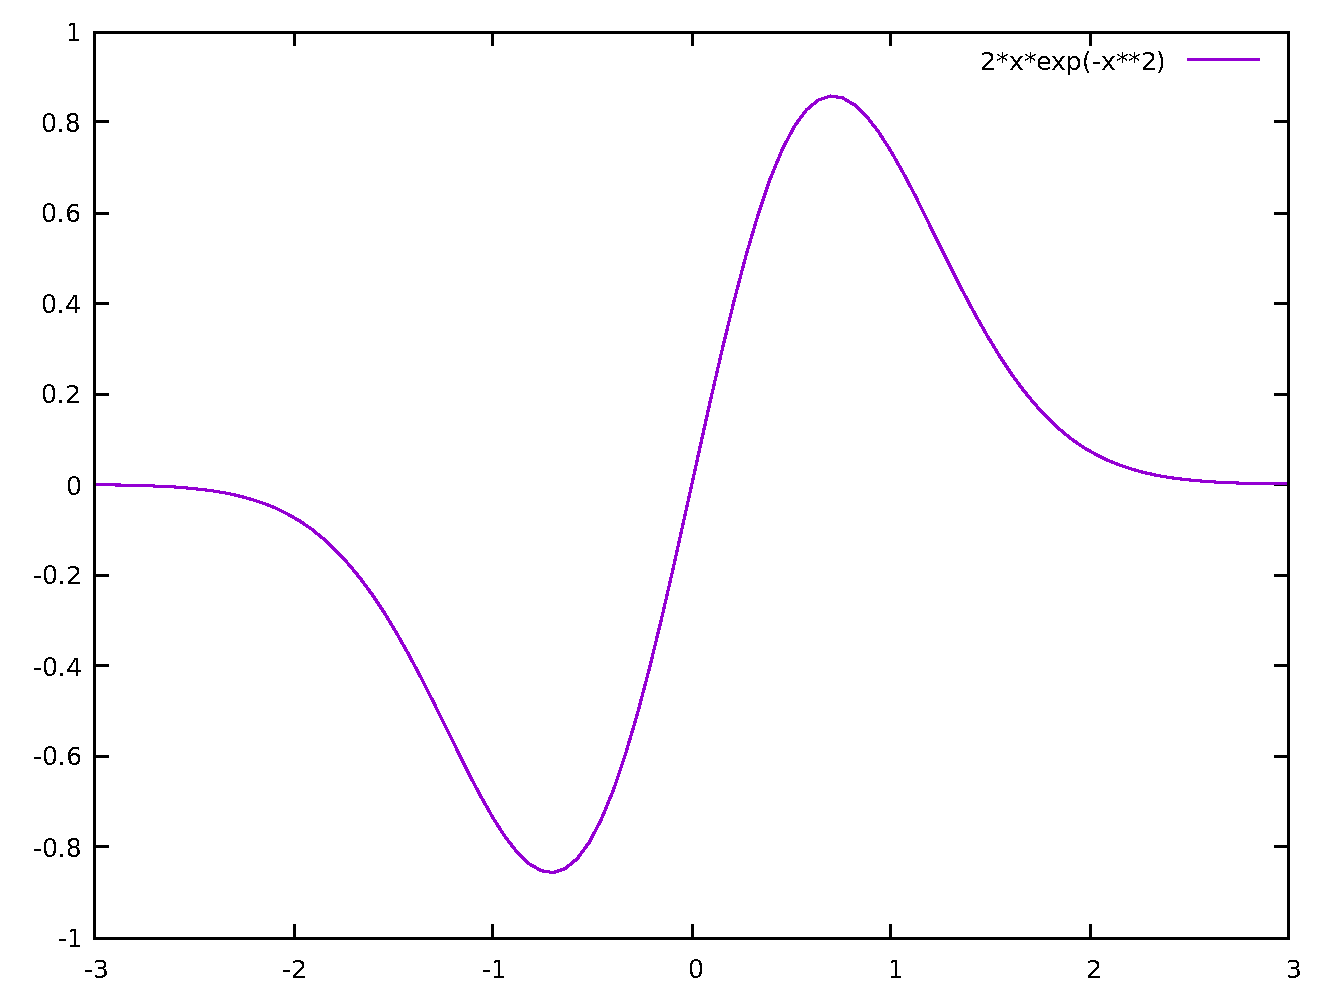
\includegraphics[width=0.6\textwidth]{desc-grad-non-conv}    
  \end{center}
  
  \begin{itemize}
  \item En partant de $x^{(0)} = 0$, on peut atteindre $-\frac{\sqrt{2}}{2}$, le minimum.
  \item En partant de $x^{(0)} = 1$, on a $x^{(k)} \rightarrow \infty$ quand $k \rightarrow \infty$. 
  \end{itemize}
  
\end{frame}


% ----------------------------------------------------------------------
\begin{frame}
  \frametitle{Longueur du pas}

  \begin{block}{De nombreuses méthodes pour déterminer $\lambda^{(k)}$}
  \begin{itemize}
  \item fixé par l'utilisateur %(normalisé par la norme du gradient)
  \item $1 / k \|{\nabla f}(x^{(k)})\|$ (le pas diminue au fur et à mesure des itérations)
  \item \emph{Newton}: $\Big( {\nabla^2 f}(x^{(k)}) \Big)^{-1}$
    \begin{itemize}
    \item $x^{(k+1)}$ est l'optimal d'une approximation quadratique en $x^{(k)}$
    \item nécessite le hessien (et le gradient)
    \end{itemize}
  \item \emph{Steepest descent}: tel que $f(x^{(k)} - \lambda^{(k)} {\nabla f}(x^{(k)}))
    = \min_{\lambda \geq 0} f(x^{(k)} - \lambda {\nabla f}(x^{(k)}))$
  \end{itemize}
  \end{block}
\end{frame}

% ----------------------------------------------------------------------
\begin{frame}
  \frametitle{Méthode de Newton: convergence en un pas}

  \begin{itemize}
  \item $f(x_1,x_2) = a_1x_1^2 + b_1x_1 + c_1 + a_2x_2^2 + b_2x_2 + c_2$
  \item 
    $\forall (x_1,x_2), \ {\nabla f}(x_1,x_2)^T = (2a_1x_1 + b_1,2a_2x_2 + b_2)$
  \item 
  $ \forall (x_1,x_2), \ \nabla^2f(x_1,x_2) =
  \left(\begin{array}{cc}
    2a_1 & 0 \\
    0 & 2a_2 \\
  \end{array}
  \right)
  $
  %
  \end{itemize}

  \begin{itemize}
  \item $\left( \begin{array}{c} x_1^{(1)} \\ x_2^{(1)} \end{array} \right ) =
    \left( \begin{array}{c} x_1^{(0)} \\ x_2^{(0)} \end{array} \right ) -
  \left(\begin{array}{cc} \frac{1}{2a_1} & 0 \\ 0 & \frac{1}{2a_2} \\ \end{array} \right) \cdot
  \left( \begin{array}{c} 2a_1x_1^{(0)} + b_1 \\ 2a_2x_2^{(0)} + b_2 \end{array} \right ) =
  \left( \begin{array}{c} -\frac{b_1}{2a_1} \\ -\frac{b_2}{2a_2} \end{array} \right ) $, or
  ${\nabla f}(-\frac{b_1}{2a_1}, -\frac{b_2}{2a_2})$ est nul : on a le minimum
  \item convergence en une itération car $f$ est quadratique
  \end{itemize}
  
\end{frame}

% ----------------------------------------------------------------------
\begin{frame}
  \frametitle{Méthode de Newton: non convergence}

  \begin{itemize}
  \item $f(x) = \left \{
    \begin{array}{ll}
      -4x^3 + 3x^4 & \text{si} \ x\geq 0 \\
      4x^3 + 3x^4 & \text{si} \ x < 0 \\
    \end{array} \right.$
  \end{itemize}
  
  \begin{center}
      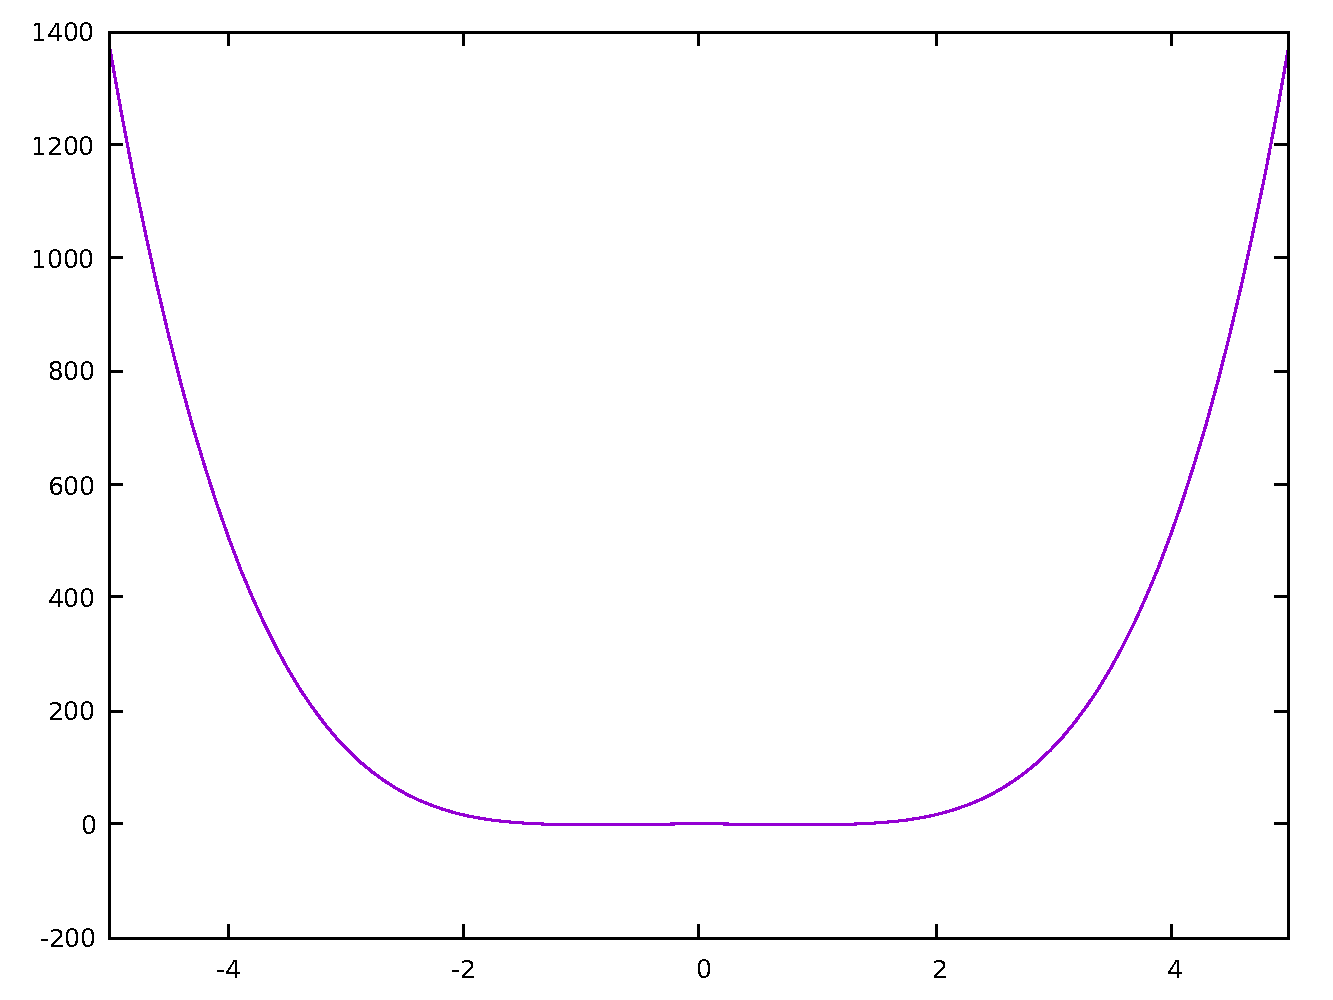
\includegraphics[width=0.6\textwidth]{newton-non-conv}    
  \end{center}
  
  \begin{itemize}
  \item En partant de $x^{(0)} = 0.4$, on converge vers 0, le minimum.
  \item En partant de $x^{(0)} = 0.6$, on a $x^{(1)}$ = -0.6, $x^{(2)}$ = 0.6\dots 
  \end{itemize}
  
\end{frame}

% ----------------------------------------------------------------------
\begin{frame}
  \frametitle{\emph{Steepest Descent}: convergence lente}

  \begin{itemize}
  \item $f(x_1,x_2) = 2x_1x_2 + 2x_2 - x_1^2 - 2x_2^2$
  \item$(x_1^{(0)}, x_2^{(0)}) = (0, 0.5)$ 
  \end{itemize}

  \begin{center}
      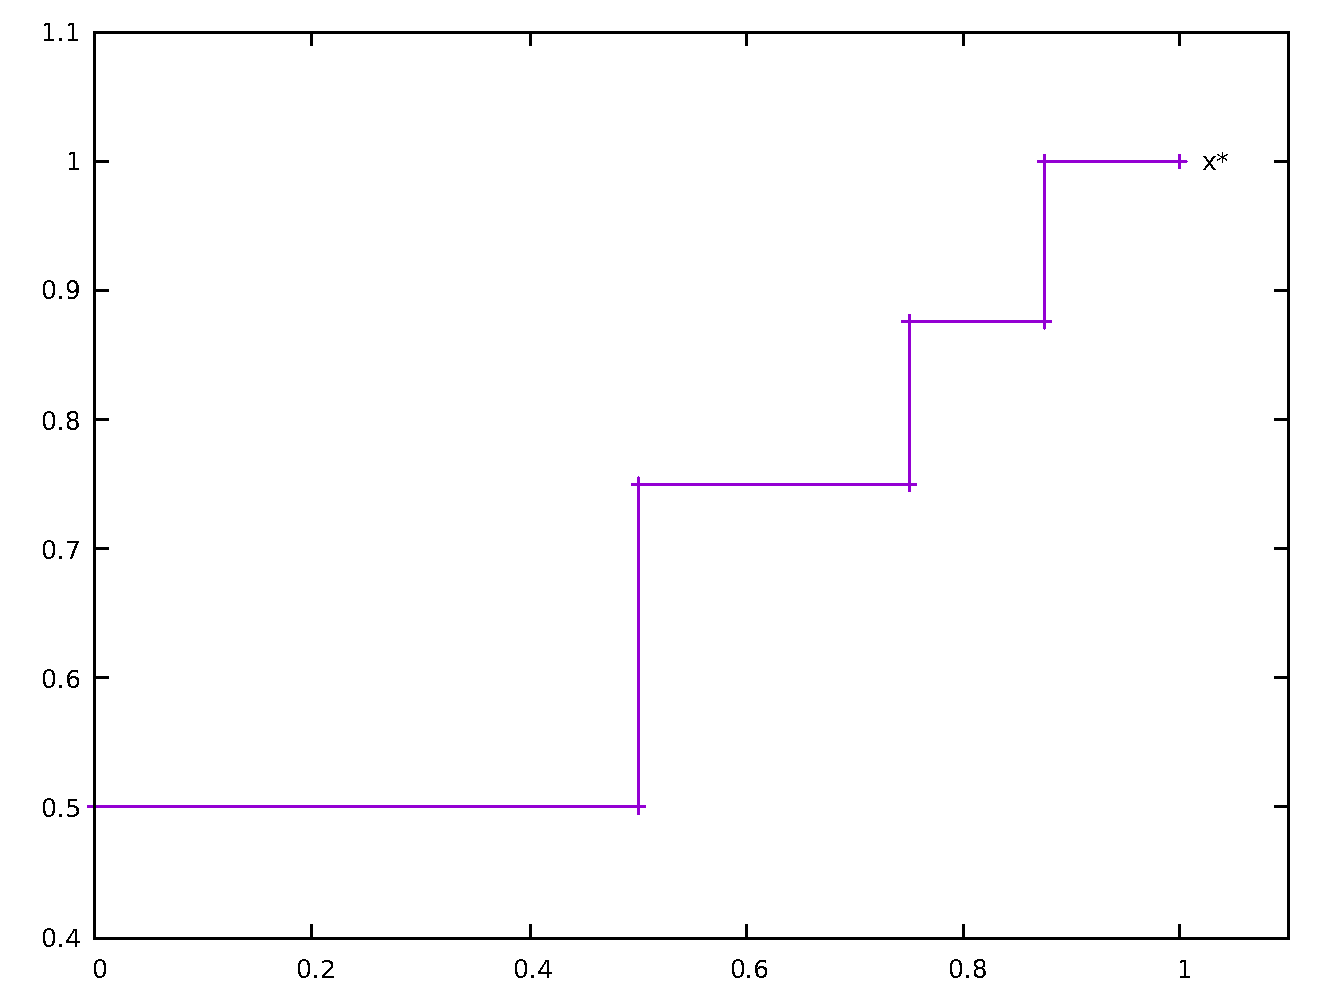
\includegraphics[width=0.6\textwidth]{steepest-desc}    
  \end{center}
  
  \begin{itemize}
  \item Deux directions successives sont toujours orthogonales
  \item Ce qui est lent pour des fonctions à \emph{vallée étroite}. 
  \end{itemize}
    
  
\end{frame}

% ----------------------------------------------------------------------
\begin{frame}
  \frametitle{Autres méthodes}

  \begin{itemize}
  \item Newton modifié et quasi-Newton
  \item méthode du gradient conjugué, méthode de Fletcher et Reeves
  \item méthode de Davidon-Fletcher-Powell (DFP)
  \item méthode de Broyden-Fletcher-Goldfarb-Shanno (BFGS)
  \item algorithme de Powell (sans dérivée !)
  \item \verb!PyTorch 2.6!: Adadelta, Adafactor, Adagrad,
    Adam, AdamW, SparseAdam, Adamax, ASGD, LBFGS, NAdam,
    RAdam, RMSprop, Rprop, SGD
  \end{itemize}
  
\end{frame}

%% % ----------------------------------------------------------------------
%% \begin{frame}
%%   \frametitle{Cas d'une somme de fonctions}

%%   \[
%%   (\text{P}^\circ) \quad
%%     \text{min} \ f(x) := \sum_{i = 1}^{m} q_i(x), \ x \in \R^n
%%   \]

%%   \[ x^{(k+1)} := x^{(k)} - \lambda^{(k)} {\nabla f}(x^{(k)}), \ \lambda^{(k)} > 0, \]

%%   \[ {\nabla f}(x) = \sum_{i = 1}^{m} {\nabla q_i}(x). \]

%%   ~
  
%%   \begin{itemize}
%%   \item méthode du gradient stochastique : on évalue le gradient
%%     \begin{itemize}
%%     \item sur 1 fonction $q_i$ au hasard : ${\nabla f}(x) := {\nabla q_i}(x)$
%%     \item ou sur plusieurs (\emph{mini-batch}), mais pas sur tout $f$.
%%     \end{itemize}
%%   \end{itemize}
  
%% \end{frame}

% ----------------------------------------------------------------------
\section{Application : problème de régression}
% ----------------------------------------------------------------------

% ----------------------------------------------------------------------
\begin{frame}<beamer>
  \frametitle{Sommaire}
  \tableofcontents[currentsection]
\end{frame}

% ----------------------------------------------------------------------
\begin{frame}
  \frametitle{IA et régression}

  \begin{block}{Apprentissage automatique supervisé}

    \begin{itemize}
      \item données : $d+1$ variables $\vec{x} \in \R^d$ et $y \in \R$ observées sur $n$ individus. 
      \item phase d'apprentissage : déterminer les paramètres $(w_1, \dots, w_m)$ d'un modèle $f$
        qui calcule $y$ à partir de $\vec{x}$.
      \item phase d'inférence : étant donné une nouvelle valeur $\vec{x}_0$,
        calculer $f(w_1, \dots, w_m)(\vec{x}_0)$
        (alors que la valeur $y_0$ correspondante est inconnue). 
    \end{itemize}
  \end{block}

\end{frame}

% ----------------------------------------------------------------------
\begin{frame}
  \frametitle{Intuition dans $\R^1$ avec un modèle linéaire}

  \begin{center}
      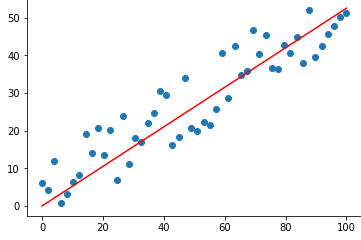
\includegraphics[width=0.5\textwidth]{linear-regression}    
  \end{center}

  \begin{itemize}
  \item en bleu, les couples $(x_i,y_i)$ observées,
  \item en rouge, le graphe de la fonction $f(w_1, \dots, w_m)$
    qui donne $y$ à partir de $x$.
  \item $m = 2$ suffit dans ce cas (pente
    et ordonnées à l'origine).
  \end{itemize}
\end{frame}

% ----------------------------------------------------------------------
\begin{frame}
  \frametitle{Régression et optimisation}

  \begin{block}{Apprentissage $=$ optimisation}

    \begin{itemize}
    \item on considère une fonction \emph{de perte} qui
      est typiquement la somme des carrés des écarts entre ce que
      donne le modèle et les observations :
      \[ L(w_1, \dots, w_m) :=
      \sum_{i=1}^n (f(w_1, \dots, w_m)(\vec{x}_i) - y_i)^2 \]
    \item on la minimise par descente de gradient
      \begin{itemize}
      \item $f$ doit être différentiable (et on doit calculer son gradient)
      \item il y a des \emph{hyper-paramètres} ($\lambda$, nombre d'itérations, etc.)
      \end{itemize}
    \end{itemize}

  \end{block}
  
\end{frame}

% ----------------------------------------------------------------------
\newcommand\mat[1]{\mathbf{#1}}

\begin{frame}
  \frametitle{Exemple de modèle}
  
  \begin{block}{Définition sous forme matricielle}
    Soit $k \in \N$.
    On a $m = k(d+2)$ paramètres stockés dans les matrices :
    \begin{itemize}
      \item $\mat{M}_1$ de taille $k \times (d+1)$,
      \item $\mat{M}_2$ de taille $1 \times k$.
    \end{itemize}
    
    \[ L(\mat{M}_1, \mat{M}_2, \mat{x}) := \mat{M}_2 \cdot \sigma ( \mat{M}_1 \cdot \mat{x} ). \]
    où $\sigma$ est une fonction d'activation non polynomiale appliquée
    élément par élément (ex. sigmoïde). 
  \end{block}
  
  \begin{block}{Théorème d'approximation universelle}
  Il existe $k$ tel qu'on approxime n'importe quelle fonction
  aussi bien qu'on veut par ce modèle ! 
  \end{block}

\end{frame}

% ----------------------------------------------------------------------
\begin{frame}
  \frametitle{Gradient ?}

  \begin{itemize}
  \item (immédiat ;-)) $\frac{\partial L}{\partial \mat{M}_2}(\mat{M}_1, \mat{M}_2, \mat{x})
    = \sigma ( \mat{x}^T \cdot \mat{M}_1^T )$
  \item (composition) on pose $\mat{z}:=\mat{M}_1\mat{x}$, $\mat{y}:=\sigma(\mat{z})$,
    \begin{align*}
    \frac{\partial L}{\partial \mat{M}_1}(\mat{M}_1, \mat{M}_2, \mat{x})
    &= \mat{M_2} \Bigg( \frac{\partial \mat{y}}{\partial \mat{z}} \frac{\partial \mat{z}}{\partial \mat{M}_1} \Bigg) \\
    &= \mat{M_2} \sigma'( \mat{M}_1 \cdot \mat{x} ) \mat{x}^T.
    \end{align*}
  \end{itemize}

  astuce : formulaire de dérivées matricielles.

  mieux : outils de dérivation automatique comme \verb!PyTorch!.
  
\end{frame}

% ----------------------------------------------------------------------
\begin{frame}
  \frametitle{Exemple de gros modèle : AlexNet (2012)}

    (CNN → RN → MP)² → (CNN³ → MP) → (FC → DO)² → Linear → softmax

où

\begin{itemize}
\item     CNN = convolutional layer (with ReLU activation)
\item     RN = local response normalization
\item     MP = maxpooling
\item     FC = fully connected layer (with ReLU activation)
\item     Linear = fully connected layer (without activation)
\item     DO = dropoutTODO
\end{itemize}

60 millions de paramètres 

\end{frame}

% ----------------------------------------------------------------------
\section{Optimisation continue avec contraintes}
% ----------------------------------------------------------------------

% ----------------------------------------------------------------------
\begin{frame}<beamer>
  \frametitle{Sommaire}
  \tableofcontents[currentsection]
\end{frame}

% ----------------------------------------------------------------------
\begin{frame}
  \frametitle{Formulation mathématique}

  \[
  (\text{P}^\bullet) \left\{
  \begin{array}{c}
    \text{trouver} \ x \ \text{qui minimise} \ f(x) \ \text{tel que :} \\
    g_i(x) \leq 0, \ i \in I = \{1, \dots, m\} \\
    x \in \R^n
  \end{array}
  \right.
  \]

  \begin{block}{Le problème peut}
    \begin{itemize}
    \item être \emph{infaisable} :
      $X := \{ x \in \R^n \ | \ g_i(x) \leq 0, i \in I \}$,
      l'ensemble des solutions candidates est vide.
    \item être \emph{non borné} : $\exists t, v, x^0$, tels que $\lim_{t \rightarrow \infty} f(x^0 + tv) = -\infty$.
    \item avoir une ou \emph{plusieurs solutions}. 
    \end{itemize}
  \end{block}
  
\end{frame}

% ----------------------------------------------------------------------
\begin{frame}
  \frametitle{Problème infaisable}

  \begin{center}
      \includegraphics[width=0.5\textwidth]{p-infaisable}    
  \end{center}
  
\end{frame}

% ----------------------------------------------------------------------
\begin{frame}
  \frametitle{Problème non borné}

  \begin{center}
    \includegraphics[width=0.4\textwidth]{p-non-borne}    
  \end{center}

\end{frame}

% ----------------------------------------------------------------------
\begin{frame}
  \frametitle{Plusieurs solutions}

  \begin{center}
    \includegraphics[width=0.4\textwidth]{p-plusieurs}    
  \end{center}
  
\end{frame}


%% % ----------------------------------------------------------------------
%% \begin{frame}
%%   \frametitle{Saturation et cône tangent en un point $x^0 \in X$}

%%   \begin{itemize}
%%     \item Une contrainte $g_i$ est \emph{saturée} en $x^0$ ssi $g_i(x^0) = 0$
%%     \item L'ensemble des contraintes saturées en $x^0$ est
%%       $\{g_i\}_{i \in I_0}, \ I_0 := \{i \ | \ g_i(x^0) = 0 \}$
%%     \item Le cône tangent en $x^0$ est donné par le gradient des contraintes saturées en $x^0$ :
%%       $G_0 := \{ y \in \R^n \ | \ {\nabla g_i}^T \cdot y \leq 0, \ \forall i \in I_0 \}$ 
%%   \end{itemize}

%%   \begin{center}
%%       \includegraphics[width=0.45\textwidth,page=1]{cone-tangent} \hspace{0.01\textwidth}   
%%       \includegraphics[width=0.45\textwidth,page=2]{cone-tangent}    
%%   \end{center}
  
%% \end{frame}

%% % ----------------------------------------------------------------------
%% \begin{frame}
%%   \frametitle{Hypothèse de qualification des contraintes (QC)}

%%   $X$ satisfait en $x^0 \in X$ l'hypothèse (QC) ssi pour tout $\epsilon$
%%   positif suffisamment petit, la boule $B(x^0,\epsilon)$ de centre $x^0$
%%   et rayon $\epsilon$ est telle que $B(x^0,\epsilon) \cap G_0 \subset X$. 

%%   \only<1>{
%%   \begin{exampleblock}{Cas où (QC) est vérifiée en $x^0$ : }
%%   \begin{center}
%%       \includegraphics[width=0.5\textwidth,page=1]{cone-tangent}    
%%   \end{center}
%%   \end{exampleblock}
%%   }
%%   \only<2>{
%%   \begin{exampleblock}{Cas où (QC) n'est pas vérifiée en $x^0$ : }
%%   \begin{center}
%%       \includegraphics[width=0.5\textwidth,page=2]{cone-tangent}    
%%   \end{center}
%%   \end{exampleblock}
%%   }
%%   \only<3>{
%%     \begin{block}{Théorème local}
%%       $(QC)$ est vérifiée \alert{en un point $x^0 \in X$}
%%       \begin{itemize}
%%       \item si les gradients $\{ {\nabla g_i}(x^0) \}_{i \in I_0}$ des contraintes saturées en $x^0$
%%         sont linéairement indépendants
%%       \end{itemize}
%%     \end{block}
    
%%     \begin{block}{Théorème global}
%%       $(QC)$ est vérifiée \alert{pour tout $x \in X$}
%%       \begin{itemize}
%%       \item si toutes les fonctions $g_i$ sont linéaires
%%       \item ou si toutes les fonctions $g_i$ sont convexes, différentiables, et l'intérieur de $X$ n'est pas vide
%%       \end{itemize}
%%     \end{block}
%%   }
  
%% \end{frame}

% ----------------------------------------------------------------------
\begin{frame}
  \frametitle{Intuition sur les conditions d'optimalité}

  \begin{center}
      \includegraphics[width=0.5\textwidth]{kkt}    
  \end{center}

\end{frame}

% ----------------------------------------------------------------------
\begin{frame}
  \frametitle{Hypothèses techniques}

  \[
  (\text{P}^\bullet) \left\{
  \begin{array}{c}
    \text{trouver} \ x \ \text{qui minimise} \ f(x) \ \text{tel que :} \\
    g_i(x) \leq 0, \ i \in I = \{1, \dots, m\} \\
    x \in \R^n
  \end{array}
  \right.
  \]

  \begin{itemize}
  \item (H1) $f$ et $(g_i)_{i \in I}$ continues, différentiables
  \item (H2) $X \neq \emptyset$
  \item (QC) hypothèse de qualification des contraintes
  \end{itemize}
  
\end{frame}

% ----------------------------------------------------------------------
\begin{frame}
  \frametitle{Conditions d'optimalité de Karush, Kuhn et Tucker}

  \begin{block}{Conditions nécessaires}
    En supposant (H1), (H2), (QC), si $x^0$ est un minimum local de $(\text{P}^\bullet)$,
    alors il existe $\{\lambda_i \geq 0\}_{i \in I}$ tels que:
    \[
    (\text{KKT})
    \left\{
    \begin{array}{ll}
      -{\nabla f}(x^0) = \sum_{i \in I} \lambda_i {\nabla g_i}(x^0)
      & \text{(stationnarité)} \\
      \lambda_i g_i(x^0) = 0, \ \forall i \in I
      & \text{(complémentarité)} \\
    \end{array}
    \right.
    \]
  \end{block}

  \begin{block}{Conditions suffisantes}
    Dans le cas où, en plus, $f$ et $\{g_i\}_{i\in I}$ sont \emph{convexes},
    si les conditions (KKT) sont vérifiées pour $x^0$, alors $x^0$ est un minimum
    (global) de $(\text{P}^\bullet)$.  
  \end{block}
  
\end{frame}

% ----------------------------------------------------------------------
\begin{frame}
  \frametitle{Exemple numérique}

  \begin{center}  
  \begin{tabular}{l}
    trouver $(x_1,x_2)$ qui minimisent \\
    \textcolor{red}{$f(x_1,x_2) := (x_1 - 3)^2 + (x_2 - 4)^2$} tels que : \\
    pour tout $i = 1,2,3$, \textcolor{blue}{$g_i(x_1,x_2) \leq 0$}, avec \\
    $g_1(x_1,x_2) := x_1 + x_2 - 5$, $g_2(x_1,x_2) := -x_1$, $g_3(x_1,x_2) := -x_2$ 
    %% \textcolor{blue}{$\left\{
    %% \begin{array}{l}
    %%   g_1(x_1,x_2) \leq 0, \ g_1(x_1,x_2) := x_1 + x_2 - 5 \\
    %%   g_2(x_1,x_2) \leq 0, \ g_2(x_1,x_2) := x_1 - x_2 - 2.5 \\
    %%   g_3(x_1,x_2) \leq 0, \ g_3(x_1,x_2) := -x_1 \\
    %%   g_4(x_1,x_2) \leq 0, \ g_4(x_1,x_2) := -x_2
    %% \end{array}
    %% \right.$}
  \end{tabular}
  \end{center}
  
  \begin{center}  
    \includegraphics[width=0.45\textwidth,page=1]{kuhn-tucker}
  \end{center}
\end{frame}

% ----------------------------------------------------------------------
\begin{frame}
  \frametitle{Résolution par les équations (KKT)}

  \only<1>{  
  \begin{itemize}
    \item Comme pour tout $x$, $\nabla^2f(x)$ est définie-positive, $f$ est convexe
    \item Les contraintes $\{g_i\}_{i \in I}$ sont linéaires donc convexes
    \item $x^\star$ et $\lambda_1,\lambda_2,\lambda_3$ qui vérifient (KKT)
      sont tels que $x^\star$ est le minimum global
    \end{itemize}
  }
  \only<2>{
    On joue aux devinette et suppose que seule $g_1$ est saturée 
  \begin{itemize}
  \item c-à-d. telle que $g_1(x^\star) = x_1^\star + x_2^\star - 5 = 0$,
  \item complémentarité : $\lambda_2 = \lambda_3 = 0$, 
  \item stationnarité : $-{\nabla f}(x^\star) = \lambda_1 {\nabla g_1}(x^\star)$.
  \end{itemize}

  Le système à résoudre est donc: 
  \[
  \left\{
  \begin{array}{l}
    x_1^\star + x_2^\star - 5 = 0 \\
  - \left( \begin{array}{c} 2x_1^\star - 6 \\ 2x_2^\star - 8 \end{array} \right) =
  \lambda_1 \left( \begin{array}{c} 1 \\ 1 \end{array} \right) \\
  \end{array}
  \right.
  \]
  D'où on déduit $x_1^\star = 2$, $x_2^\star = 3$, $\lambda_1 = 2$. 
  }

  \only<3>{
  \begin{center}  
    \includegraphics[width=0.45\textwidth,page=2]{kuhn-tucker}
  \end{center}
  }
\end{frame}

% ----------------------------------------------------------------------
\begin{frame}
  \frametitle{Méthodes d'optimisation}

  \begin{itemize}
  \item Recherche combinatoire et résolution des équations (KKT)
    %par des méthodes d'optimisation sans contrainte
    %ex. resoudre ax = b revient a minimiser (ax - b)^2  
  \item Méthodes des pénalités
    %: on élimine les contraintes en ajoutant à la fonction objectif des pénalités qui assurent
    %qu'un point $\bar{x} \notin X$ ne soit pas minimum   
  \item Méthodes exploitant la théorie de la dualité de Lagrange
    %algorithmes d'Uzawa, Arrow-Hurwicz, Dantzig, méthode des multiplicateurs 
  \item Méthodes de descente sous contrainte
    %: de la solution courante, on cherche un déplacement de descente vers un point de $X$
    %méthodes des directions réalisables, du gradient projeté, du gradient réduit (généralisé)...
  \item Méthodes de linéarisation
    %: à chaque étape, on cherche le minimum d'une approximation linéaire de $f$ pour trouver le déplacement 
    %méthode de Franck et Wolf, plans sécants de Kelley, génération de colonne de Dantzig...
  \item \dots
  \end{itemize}
  
\end{frame}

% ----------------------------------------------------------------------
\begin{frame}
  \frametitle{Note : cas particulier de fonctions linéaires}

  On appelle problème d'optimisation linéaire (ou \emph{programme linéaire}),
  le problème d'optimisation suivant : 
  \[
  \text{(PL)} \left\{
  \begin{array}{c}
    \text{trouver} \ x \ \text{qui minimise} \ f(x) \ \text{tel que :} \\
    g_i(x) \leq 0, \ i \in I = \{1, \dots, m\} \\
    x \in \R^n \\
    f, \{g_i\}_{i \in I} \ \text{sont linéaires} \\
  \end{array}
  \right.
  \]

  (PL) est résolu en pratique par la méthode du \emph{simplexe}
  %% dû essentiellement à Dantzig (1947). Le traitement correct
  %% des configurations dégénérées est dû à Bland (1977).
  %% cf. https://en.wikipedia.org/wiki/Revised_simplex_method
  ou celle \emph{des points intérieurs}.
\end{frame}

% ----------------------------------------------------------------------
\section{Application : problème de classification}
% ----------------------------------------------------------------------

% ----------------------------------------------------------------------
\begin{frame}<beamer>
  \frametitle{Sommaire}
  \tableofcontents[currentsection]
\end{frame}

% ----------------------------------------------------------------------
\begin{frame}
  \frametitle{IA et classification binaire}

  \begin{block}{Apprentissage automatique supervisé}

    \begin{itemize}
      \item données : $d+1$ variables $\vec{x} \in \R^d$ et $y \in \{-1,1\}$ observées sur $n$ individus. 
      \item phase d'apprentissage : déterminer les paramètres $(w_1, \dots, w_m)$ d'un modèle $f$
        qui détermine $y$ à partir de $\vec{x}$.
      \item phase d'inférence : étant donné une nouvelle valeur $\vec{x}_0$,
        le classifieur renvoie
        \[
        \left\{
        \begin{array}{l} 1 \ \text{si} \ f(w_1, \dots, w_m)(\vec{x}_0) \geq 0 \\
          -1 \ \text{sinon}.
        \end{array}
        \right.
        \]
    \end{itemize}
    
  \end{block}

\end{frame}

% ----------------------------------------------------------------------
\begin{frame}
  \frametitle{Intuition dans $\R^2$ avec un modèle linéaire}
  
  \centering
  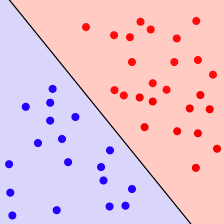
\includegraphics[width=3cm]{linear-separation.png}

  ~
  
  \begin{itemize}
  \item points rouges sont les $\vec{x}_i$ tels que $y_i = 1$, 
  \item points bleus sont les $\vec{x}_i$ tels que $y_i = -1$, 
  \end{itemize}
  
\end{frame}

% ----------------------------------------------------------------------
\begin{frame}
  \frametitle{Classification et optimisation}

  \begin{block}{Apprentissage $=$ optimisation sous contrainte}

    \begin{itemize}
    \item le classifieur ne fait pas d'erreur si, pour tout $i$,
      $y_i f(w_1, \dots, w_m)(\vec{x}_i) > 0$ : c'est un ensemble
      de contraintes.
    \item la fonction objectif est typiquement 
      \[ L(w_1, \dots, w_m) := w_1^2 + \dots + w_m^2, \]
      ce qui revient à maximiser la marge de séparation
    \end{itemize}
  \end{block}

  \begin{block}{SVM}
    C'est le principe des séparateurs à vaste marge (SVM),
    un temps à la mode du fait d'une plus grande capacité de
    généralisation que les réseaux de neurones. 
  \end{block}
      
\end{frame}

%% % ----------------------------------------------------------------------
%% \section{Optimisation discrète}
%% % ----------------------------------------------------------------------

%% % ----------------------------------------------------------------------
%% \begin{frame}<beamer>
%%   \frametitle{Sommaire}
%%   \tableofcontents[currentsection]
%% \end{frame}

%% % ----------------------------------------------------------------------
%% \begin{frame}
%%   \frametitle{Problème d'optimisation linéaire en nombre entiers}
  
%%   \[
%%   \text{(PNE)} \left\{
%%   \begin{array}{c}
%%     \text{min} \ f(x) \ \text{tel que :} \\
%%     g_i(x) \leq 0, \ i \in I = \{1, \dots, m\} \\
%%     x \in \alert{\Z^n}
%%   \end{array}
%%   \right.
%%   \]

%%   \begin{block}{Hypothèses habituelles}
%%     \begin{itemize}
%%     \item L'ensemble des solutions candidates
%%       $X := \{ x \in \Z^n \ | \ g_i(x) \leq 0, i \in I = \{1, \dots, m\} \}$ \\
%%       est borné et non vide
%%     \item $f, \{g_i\}_{i \in I}$ sont \emph{linéaires} \\
%%       (il existe beaucoup d'astuces pour
%%       linéariser le problème en introduisant des variables supplémentaires)
%%     \end{itemize}
%%   \end{block}
%% \end{frame}

%% % ----------------------------------------------------------------------
%% \begin{frame}
%%   \frametitle{De nombreux problèmes se ramènent à (PNE)}

%%   \begin{itemize}
%%     \item problème d'affectation (assignment problem)
%%     \item problème des surveillants de musée (art gallery problem)
%%     \item problème de coloration (graph coloring)
%%     \item problème du sac à dos (knapsack problem)
%%     \item problème du voyageur de commerce (travelling salesman problem)
%%     \item problème de séquençage de tâches (job sequencing)
%%     \item \dots
%%   \end{itemize}
  
%% \end{frame}

%% % ----------------------------------------------------------------------
%% \begin{frame}
%%   \frametitle{Un problème différent de sa relaxation continue}

%%   \only<1>{
%%   \alert{L'optimum entier est aussi éloigné qu'on veut de l'optimum continu}

%%     \[
%%     \left\{
%%     \begin{array}{c}
%%       \text{min} \ -10x_1 - 11x_2 \ \text{tel que :} \\
%%       10x_1 + 12x_2 \leq 59, \ x_1 \geq 0, \ x_2 \geq 0 \\
%%     \end{array}
%%     \right.
%%     \]

%%     \begin{center}
%%       \includegraphics[width=0.5\textwidth]{ex-plne}
%%     \end{center}
%%   }

%%   \only<2>{
%%     \begin{block}{Cela change complètement le problème !}
%%       \begin{itemize}
%%       \item (PL) est un problème polynomial,
%%         l'algorithme du simplexe (bien qu'exponentiel au pire cas)
%%         est même plutôt efficace en pratique, 
%%       \item (PNE) est un problème NP-complet
%%       \end{itemize}
%%     \end{block}
%%   }
%% \end{frame}

%% % ----------------------------------------------------------------------
%% \begin{frame}
%%   \frametitle{Méthodes de résolution}

%%   \begin{itemize}
%%   \item recherche exhaustive (très-très petits problèmes),
%%   \item \emph{Branch and Bound} (séparation-évaluation)
%%   \item relaxation continue dans certains cas particuliers
%%   \item méthode des coupes (intégrales, mixtes)
%%   \item \emph{Branch and Bound} + coupes $=$ \emph{Branch and cut}
%%   \item programmation par contraintes
%%   \item méta-heuristiques : \\
%%       glouton, meilleur voisin, tabou, recuit-simulé, algorithme génétique, colonie de fourmis, \dots
%%   \end{itemize}
  
%% \end{frame}


% ----------------------------------------------------------------------
\section{Conclusion}
% ----------------------------------------------------------------------

% ----------------------------------------------------------------------
\begin{frame}<beamer>
  \frametitle{Sommaire}
  \tableofcontents[currentsection]
\end{frame}

% ----------------------------------------------------------------------
\begin{frame}
  \frametitle{Différentes classes de problèmes et d'algorithmes}

  \[
  \text{(P)} \left\{
  \begin{array}{c}
    \text{trouver} \ x \ \text{qui minimise} \ f(x) \ \text{tel que :} \\
    g_i(x) \leq 0, \ i \in I = \{1, \dots, m\} \\
    x \in S \subseteq \R^n
  \end{array}
  \right.
  \]

  \begin{itemize}
  \item Optimisation continue ($S = \R^n$)
    \begin{itemize}
    \item sans contrainte ($I = \emptyset$) \\
      \emph{descente de gradient}
    \item avec contraintes ($I \neq \emptyset$) 
      \begin{itemize}
        \item non-linéaires
        \item linéaires \\
        \emph{simplexe, points intérieurs}
      \end{itemize}
    \end{itemize}
  \item Optimisation combinatoire ($S = \Z^n$)\\
    \emph{branch and bound}, \emph{(meta)-heuristiques} 
  \end{itemize}
  
\end{frame}

% ----------------------------------------------------------------------
\begin{frame}
  \frametitle{Lien avec l'IA}

  \begin{block}{Exemple de l'apprentissage automatique supervisé}

    \begin{itemize}
      \item données : $d+1$ variables $\vec{x} \in \R^d$ et $y$ observées sur $n$ individus. 
        \begin{itemize}
        \item si $y \in C$ variable \emph{catégorielle}, problème de \emph{classification}. 
        \item si $y \in \R$ variable \emph{quantitative}, problème de \emph{régression}. 
        \end{itemize}
      \item phase d'apprentissage : déterminer les paramètres $(w_1, \dots, w_m)$ d'un modèle $f$
        qui calcule $y$ à partir de $\vec{x}$.
      \item phase d'inférence : étant donné une nouvelle valeur $\vec{x}_0$,
        déterminer une valeur $y_0$ à partir de $f(w_1, \dots, w_m)(\vec{x}_0)$. 
    \end{itemize}
  \end{block}

\end{frame}

%% % ----------------------------------------------------------------------
%% \begin{frame}
%%   \frametitle{Pour aller plus loin}

%%   \begin{itemize}
%%   \item Théorie de la dualité de Lagrange
%%   \end{itemize}


%%   \begin{itemize}
%%   \item Livre de référence sur les aspects théoriques de l'optimisation
%%   \end{itemize}

%% \begin{thebibliography}{alpha}
%% \bibitem{MM}
%% Michel Minoux, \emph{Programmation mathématique, Théorie et algorithmes}, Lavoisier, 2eme édition, 2008, 711 pp.
%% \end{thebibliography}

%% \end{frame}

\end{document}

